\chapter{Theoretical Framework for Code Refactoring}

\section{Background}
\label{sec:background}

% ---
% Defining Refactoring
% ---

% Intro
Refactoring is a well established concept in software development.
Especially in complex projects, 
	tasks like cleaning and restructuring code are regularly occurring and often times necessary. 
When referring to these activities by name, many employees use the term refactoring. 
The exact definition of the term \emph{refactoring} is not always self-evident,
	despite its familiarity.
To avoid referring to the term too loosely, 
	it is consequently important to give a precise definition as a reference for this thesis. 

% Fowler Refactoring Definition
Martin \textcite[p. ~xiv]{fowler2018} managed to formulate a definition that is both short and precise. 
He is one of the most prominent figures in the field of refactoring, 
	and has pioneered many concepts, which this thesis is going to discuss.
Fowler defines refactoring in the following:
\begin{quote}
\textbf{Refactoring} is the process of changing a software system in a way 
	that does not alter the external behavior of the code yet improves its internal structure.
\end{quote}

% Definition in Own Words
According to this definition, 
	refactoring should not change the features of the program.
By proper refactoring, 
	we can thus alleviate the risk associated with changing the codebase, 
    such as the creation of new bugs.

% --
% Refactoring Example
% --

% ---
% Objective: Explain External behavior and Internal Structure
% TODO: Refer to example
% ---

\clearpage
\subsection{Benefits: Why should we refactor?}

% Adding Features is attractive
The benefit of refactoring is not as obvious as other activities in software development. 
Spending valuable resources on a process that does not add new functionality, 
	might sound unappealing to many managers and software engineers.
Likewise, \textcite[p.~1]{kim2012} add the problem of not sensing an immediate benefit when refactoring.
Furthermore, the value of improving the internals of the code is hard to show to a manager, 
	who is not an expert and even harder to present to the client, who is paying for the work.

Having said that, when refactoring is ignored, there is not necessarily more time available.
Through continuous modifications and adaptations to new requirements, 
	the code becomes increasingly complex and drifts away from the original design.
By not improving the quality of the software, which would counteract this complexity, 
	a major part of the resources is still spent on software maintenance (\cite[p.~1]{mens2003}). 

% Refactoring necessary to avoid maintenance costs
Having Fowler's Definition in mind, 
	we thus aim to mitigate time spent on tedious maintenance, 
	and rather improve the quality attributes of the code beforehand.
Neglecting such work, would increase debt, 
	which would have to be repaid in the future in the form of costly maintenance costs.
Moreover, by obtaining this so-called \emph{technical debt}, 
	future features are more expensive to implement, and sudden changes are near impossible. 
The concept of technical debt is important to fully grasp, 
	which is why it is further explained in a future section of this thesis
(see Section \ref{sec:Business}).


% Internal Structure = Improving the Quality Attributes
In general, refactoring helps to improve the internal quality attributes of the software (\cite[p.~129]{mens2004}). 
For instance, some refactorings remove code redundancy, 
	some raise the level of abstraction, 
	some enhance the reusability, and so on.
\textcite{bass1998} distinguishes
	between two types of quality attributes. 
One type is concerned with the observation of the system at runtime, 
	such as performance and security, 
	whereas the other type does not consider  system runtime.
During refactoring, we are mostly concerned with the latter, 
	meaning we ignore the performative aspect of software during runtime.

% Listing Attributes
During a study on the value of quality attributes on refactoring, 
	\textcite[p.~4]{alkhazi2020} identified 
	six of such quality attributes: 
	Reusability, Flexibility, Understandability, 
	Functionality, Extendibility, and Effectiveness.
We will not go into detail of each attribute, 
	but it is still important to remember some of them,
   to measure whether the refactoring improved the internal quality of the software.
In addition, choosing the relevance of quality attributes,
	highly depends in particular on the project at hand.
Fortunately, even without understanding the specificities of these attributes,
	programmers can get a feel of what code with high quality is.
As a rule of thumb, 
	if it takes the programmer a week to make a change 
	that would have taken only an hour with proper quality, 
	we can assume that most of these attributes are at 
	least partly not fulfilled.

% Interconnectedness
The advantage of knowing quality attributes, is the ability to evaluate refactorings. 
In particular, the effect of a refactor can be estimated, 
	by the level of improvement in these quality attributes.
Again, the transformation of the internal structure 
	is the deciding factor on which success is measured.
Refactoring adds value if at least one quality attribute has significantly improved.

% External Structure = Tests
As previously mentioned, there is one requisite when measuring the added value.
The external behavior must not altered. 
As an example, changing the code base could make the program more modular, 
	but during the process create bugs that didn't exist before. 
Accordingly, to make meaningful evaluations, 
	it must be proven that only the internal structure has changed.
This can be achieved by writing software tests beforehand 
	and then testing the features after the refactor.
Consequently, software tests is a major component when deciding the success of a refactor.


% ---
% Criteria: When should we Refactor
% ---

\subsection{Criteria: When should we Refactor?}

% Critical Perspective
From a business standpoint, there needs to be little to no explanation, 
	when debating time spent on new features and fixing unresolved bugs.
As discussed earlier, it is significantly harder to persuade doing a refactor, 
	as there are fewer immediate benefits.
For that reason, one needs to verify the necessity of a refactor 
	and compare it to the need of other pending tasks.
\textcite[p.~5]{fowler2018} points out that if the code works and doesn't ever need to change, 
	it's fine to leave it alone.
He suggests that as soon as someone needs to understand how the code works, 
	and struggles to follow it, one has to do something about it.
Accordingly, a potential improvement in quality, doesn't warrant a refactor by itself.

% Small Refactors
It is crucial to note that refactoring does not have to be a massive, obscure undertaking.
Even if there is a demand for a huge refactor, the refactorings themselves are minor.
Refactoring is all about applying small behavior-preserving steps 
	and making a big change by stringing together a sequence of these behavior-preserving steps (\cite[p.~45]{fowler2018}). 
For this reason, refactoring as a principle, 
	always plays a key role in software development, 
	as code being easier to understand and cheaper to modify is vital.
Therefore, with projects that appear to be qualitatively sufficient, 
	active monitoring of the code quality and continuous improvements 
	through refactorings are still advisable.

% Two Hats
This approach leads to the presumption that these activities can be done in parallel.
It is, however, important to note, 
	that this parallelism doesn't suggest that one can add features and refactor at the same time.
The interplay between them can be described making use of an analogy (\cite[p.~47]{fowler2018}). 
Fowler sees software development as wearing two hats, 
	proposing that time is divided between adding functionality and refactoring. 
He argues that these activities should be distinctively separated, 
	meaning that during a refactor one should not add functionality and vice versa. 
To support his point, 
	Fowler adds that “often the fastest way to add a new feature is to change the code to make it easy to add” (\cite[p.~53]{fowler2018}) 
Conversely, once the code is better structured, 
	time can be efficiently spent on adding new capabilities.

% Transition
This approach illustrates nicely that refactoring 
	should be an integral part of software development according to Fowler's standpoint.  
Moreover, it challenges the frequent notion of refactoring being 
	cleaning up quality deficient code and fixing past mistakes. 

% Planned Refactor
Once the relationship between refactorings and adding features is understood, 
	one can better estimate the timing of each activity.
Even though we learned that refactoring at its best is fairly small, 
	by understanding the precise relationship, 
	we can argue that planned refactoring is not always a mistake.
In more concrete terms, if we agree that better structured code 
	allows us to add features quicker, 
	we can infer that there could be moments where dedicated time spent on refactoring 
	is necessary to get the code base into a better state for new features (\cite[p.~53]{fowler2018}).

% ... compared to small steps
Contrasting large and potentially complex refactors with our previous definition of 
	refactoring being smaller steps, we realize 
	that there exists a difference in scope.
The difference in scope being precisely 
	the amount of small refactoring steps needed to be applied.
Therefore, with certain projects, doing continuous refactoring during the development process might not suffice, 
	and an overarching refactor is necessary.

% Transition: Critical view
According to these presumptions, the conclusion would be 
	that with increased code quality small refactors suffice, 
	whereas with a lack of code quality larger refactorings are required. 
Although this is typically valid, there are exceptions one needs to keep in mind. 
Indeed, there are scenarios, which challenge both assumptions.

% Arguments: Transformation 
The assumption that small and continuous refactor suffice, for code bases with high quality, 
	does not hold if one of the quality attributes gains significantly in importance, 
Such a situation could justify a larger refactor of code, 
	even though it is perceived as being high in quality. 
This is typically the case,
	with approaching of large transformations to the code base. 
For example, unprecedented security risks might demand the code base 
	to be more testable.
Another case would be a migration to the cloud, which would require the code being high in modifiability. 
Consequently, a larger refactoring would then be used to satisfy these requirements.

% Argument: Lack of importance
The second assumption was that code that clearly lacks quality 
	would inevitably result in a lot of time spent in refactoring.
In contrast, 
	if a part of code is relatively insignificant,  
	an argument for a planned refactoring is difficult 
	to be made when accounting the associated costs. 
Here, minor restructurings and bug fixes could suffice. 
However, once the part gains in importance, 
	a larger refactoring could then be considered and might be necessary. 
This means that successful refactoring can also be thought of 
	allocating the companies' resources efficiently. 
Having a business case for refactoring is such an important topic, 
	that it will be discussed later in section (X).

% Conclusion
In summary, it is safe to say 
	that large refactoring efforts and tedious maintenance in post is not desirable. 
This is because ignoring refactoring, even though it is required,
	will result in costs and risks.
The ideal case is, then, 
	that decisions are conducted in advance 
	by establishing refactoring as an integral part 
	of the software development process.
Refactor can then be thought of as a 
	potential investment that would be repaid in the future. 

% ---
% 3 Key Benefits: Why Should we Refactor
% ---

% \subsection{Benefits}

% We now have a thorough understanding 
% 	of the timing of the refactor. 
% The previous sections implied the overarching reason of refactoring, 
% 	which is the increase of code quality. 
% However, 
% 	we did not formulate the concrete benefits. 
% By asking ourselves why we should refactor, 
% 	we can better understand the scope and complexity of a refactor. 
% In addition, one might realize that 
% 	small changes during the development phase can suffice 
% 	in avoiding software decay in the future.
% Fowler \textcite[p.~47]{fowler2018} states three key benefits that answer the question of why exactly we should refactor.

% ---
% Challenges: What to watch out?
% ---

\subsection{Challenges: What to watch out?}

% Intro
With a thorough understanding of the complexities 
	such as benefits, scope and timing of refactoring, 
	the effective act of refactoring seems fairly easy in comparison. 
In other words, 
	the actual difficulties
	might be related to the planning rather than the implementation. 

% Two hats
% Note: Could be shortened
The difficulties of planning become even more evident,
	when working within teams.
Going back to the analogy of the two hats, 
	we assumed that the software development process 
	is conducted by an individual. 
In practice, however, 
	the development is typically done with more than one person. 
 This makes refactoring considerably more difficult,
 	knowing that refactoring and adding new features 
	should be a distinct activity. 
Thus, a programmer decides to refactor in a team,
	said programmer could inhibit others from working on the code 
	at the same time. 
In other words, it is particularly easy to swap hats when coding alone, 
	but much more difficult when the coding is done in teams. 
As a result, 
	it is a challenge to clearly separate 
	which part of the code base is being refactored, 
	and which is added functionality. 
The underlying goal is to reach a state,
	where the separate parts are entirely independent. 
When ignoring this division, 
	the risk of bugs being introduced becomes much higher. 
As a consequence, 
	the essential premise of refactoring, 
	being that no observable behavior is changed, 
	cannot be achieved.

% Counterintuition
These challenges related to refactoring 
	may sound intimidating and time-consuming at first.
Fowler \textcite[p.~56]{fowler2018} argues against this belief,
	by suggesting that the whole purpose of refactoring 
	is to speed things up.
The key is, as with most software-related work, to not do it blindly, 
	and try to do the refactoring with intent.
 This means to not only focus on the practical steps of refactoring,
 	but also to always have an overview of the entire project.
Situating refactoring within the broader scale of the project 
	allows to actively decrease risks and 
    enables to focus on the overall quality of the code base.
Even though refactoring is often done on a small scale,
	its effects can be examined 
	throughout the layers of the software architecture.
This is especially apparent when incrementally improving previously discussed attributes,
	such as Extendibility, Reusability, and Flexibility, 
	which in turn affect the whole state of the project. 

% Conclusion: Competence
In practice, 
	“too little refactoring is far more prevalent than too much” 
	(\cite[p.56]{fowler2018}).
The suggestion that people should attempt to refactor more often, 
	is, however, much easier said than done.
Besides the mentioned challenges, 
	refactoring can add considerable value, 
	with the precondition that it is properly carried out.
Carrying out refactorings, however, is not always an easy task, 
	requires education, and most definitely experience.
This can indeed be seen as another challenge, 
	which depends on the competences of the software engineers who are actively involved.

% Transition

% In addition, on a broader level, the team, 
% 	or company must be aware of the trade-offs relating to refactoring. 
% Refactoring is dynamic in its nature,
% 	as the quality of the code and the overall objectives,
% 	must constantly be reassessed,
% 	in order for the refactoring to be most effective.
% These associated trade off between opportunities and risks, 
% 	and also costs and benefits, are 
% 	primarily relevant in business thinking. 
% Regarding the importance of investing resources into refactoring, 
% 	this tehsis will spend some time 
% 	looking at the business case of refactoring.
% The following part will set out to answer questions such as

% [...]

% --
% Code Smells
% --

\section{Formalization of Code Smells}

% Transition: Relationship between Refactoring and Code Smells
Knowing just the importance and applications of refactoring does not suffice, 
	as one still needs to understand the indications 
	that lead to an individual refactoring.
\textcite[p.~71]{fowler2018} argues that deciding when to start refactoring,
	and when to stop,
	is just as important to refactoring,
	as knowing how to operate the mechanics of it.
Particularly, there is no clear-cut moment when to refactor, 
	there are only indications 
	that there is trouble that can be solved by a refactoring.
In practice, 
	these indications are known as code or design smells 
	(\cite[p.~2]{lacerda2020}).
These two terms are distinguished by being either located at a lower level,
	known as the code level, or on a higher level, 
	the design level. 
Hence, 
	depending on the degree of complexity, 
	the smells are named code smell or design smell.
As throughout this work we are not concerned 
	with design decisions of the codebase, 
	we will from now on refer to the indications as code smells.

% What is a Code Smell?
The term “smell” is used in reference to an internal software problems
	\textcite[p.~2]{lacerda2020}, 
	which can negatively impact software quality 
	(\cite[p.~1]{sonnleithner2021}). 
One might think that software bugs fall into this category, 
	but this is a false assumption.
Although bugs also negatively impact the state of software, 
	code smells do not necessarily cause the application to break.
Nonetheless, these internal problems may lead to other negative consequences,
	such as the “impacting on software maintenance and evolution”
	\cite[p.~2]{lacerda2020}.
 
% Illustration
\begin{figure}[htp]
    \centering
    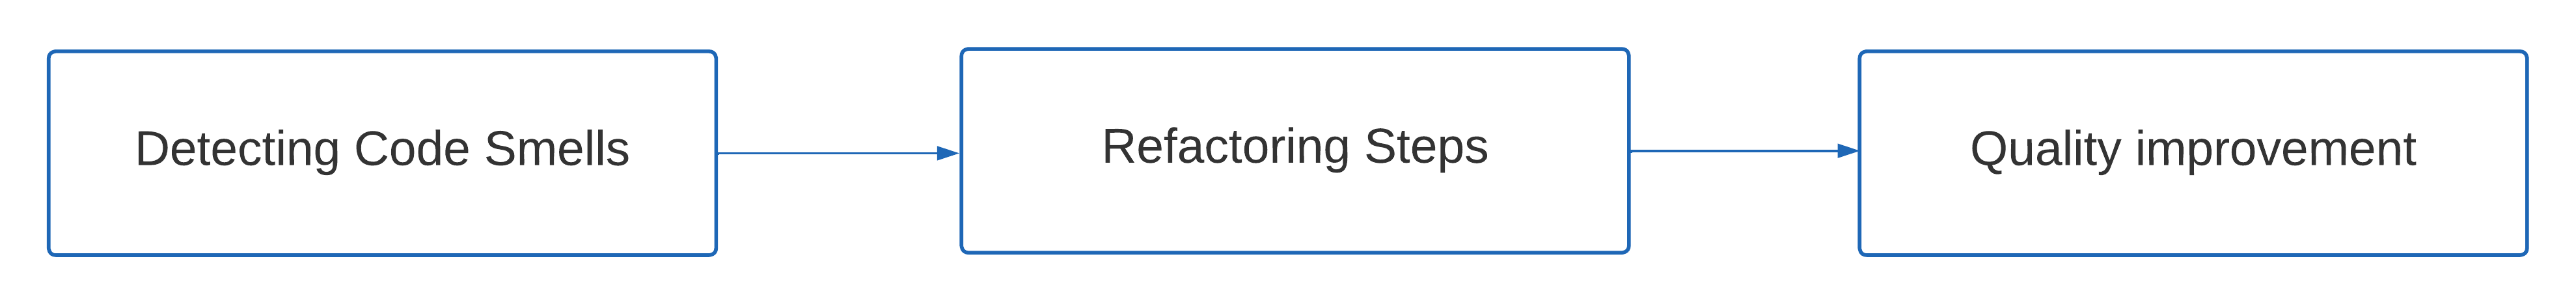
\includegraphics[width=\textwidth]{./assets/simple_process.png}
    \caption{Simplified model of Refactoring}
\end{figure}

% Connection
Knowing that code smells refer to internal problems,
	it becomes apparent that they are linked to refactoring, 
	which tries to improve the internal state of the software.
In other words, 
	refactoring can be thought of getting rid of code smells. 

% Examples Intro
To better comprehend these code smells, it is best to list some of them. 
However, to stay within the scope of this thesis, 
	we will limit the examples to the most prominent ones. 
In their work, Fowler and Beck introduced a total of 24 code smells to avoid.
Therefore, 
	the following overview briefly summarizes 
	the top ten most frequently reported code smells according to 
	[p.~15]\textcite{lacerda2020}.

% Table
	% TODO: Need to be in list of figures, right?
\subsection{Code Smells}
\label{sec:smells}

Summary of code smells identified by Fowler and Beck \textcite{fowler2018} 

\newcolumntype{b}{X}
\newcolumntype{s}{>{\hsize=.5\hsize}X}
\renewcommand{\arraystretch}{1.7}
\scalebox{0.8}{
\begin{tabularx}{1.2\textwidth}{{sb}}
	Code Smells & Description \\
 \hline
	Duplicated Code & Consists of equal or very similar passages in different fragments of the same code base.  \\
	Large Class & Class that has many responsibilities and therefore contains many variables and methods. \\
	Feature Envy & When a method is more interested in members of other classes than its own,
		is a clear sign that it is in the wrong class \\
	Long Method & Very large method/function and, therefore, difficult to understand, extend and modify.
		It is very likely that this method has too many responsibilities,
		hurting one of the principles of a good OO design \\
	Long Parameter List & Extensive parameter list, which makes it difficult to understand
		and is usually an indication that the method has too many responsibilities. \\
	Data Clumps & Data structures that always appear together,
		and when one of the items is not present, the whole set loses its meaning \\
	% Refused Bequest & It indicates that a subclass does not use inherited data or behaviors \\
	Divergent Change & A single class needs to be changed for many reasons.
		This is a clear indication that it is not sufficiently cohesive and must be divided \\
	Shotgun Surgery & Opposite to Divergent Change,
		because when it happens a modification, several different classes have to be changed \\
	Lazy Class & Classes that do not have sufficient responsibilities and therefore should not exist \\
\end{tabularx}
}

% Conclusion (Transition)
Despite having an infinite amount of potential code smells,
	the list gives a good overview of internal problems.
Being aware of these pattern is crucial
	in order to achieve the goals of improving the state of software quality.
Ignoring these smells might not seem to be that big of a problem. 
In cumulation, 
	however, getting rid can have a significant effect.
Furthermore, 
	looking at it from a broader perspective, 
	code decay inhibits the software development project. 
Refactoring then becomes a tool for programmers to invert this decay.
If ignored, 
	this effect becomes harder and harder to manage, 
	as it is increasingly difficult to both change the internal state and 
	add features, with software that is lacking quality. 
This is why it is essential not to do refactorings in stages, 
	but in a simultaenous manner.
Disregarding this, 
	leads to the accumulation of debt, 
	which is formaly known as technical debt. 
The concept of technical debt will be the main theme 
	in the following part, 
	which focusses on the business case of refactoring.

% Conclusion (1)
Despite having an infinite amount of potential code smells,
	the list gives a good overview of possible internal problems.
Being aware of such pattern is crucial
	to improve the state of software quality.
The act of ignoring a code smell, 
	might not seem to be that big of a problem at first. 
Cumulatively, however, 
	getting rid of smells does have a significant effect.
From a broader perspective, not acting on int12340ernal problems results in
	code decay, which in turn inhibits the software development project. 

% Conclusion (2)
Refactoring then becomes a tool for programmers to be able to invert code decay.
In other terms, 
	neglecting code smells becomes harder and harder to manage, 
	as it is increasingly difficult to both change the internal state and 
	add features, with software that is lacking quality. 
This is why it is essential not to do refactorings in stages, 
	but in a simultaneous manner.
Disregarding this, 
	leads to the accumulation of debt, 
	which is formally known as technical debt. 
The concept of technical debt will be the main theme 
	in the following part, 
	which focuses on the business case of refactoring.

\chapter{The Business Case for Refactoring}
\label{sec:Business}

% Introduction
During the lifetime of a project, one has to inevitably deal with internal problems appearing in the software systems. While having these code smells in our programs, the company has to suffer in terms of costs that we can only be mitigated by getting rid of the smells by refactoring.  A prototypical example of a common financial cost is the additional time spent, whilst programming with deficient code. Naturally, employees are spending less time when their code is easy to read, understand, and modify. Conversely, through the accumulation of code smells in software systems, companies are exposed to a financial burden they might want to get rid of. Examining this discussion between code smells  and financial costs paves the way to consider refactoring decisions from a business standpoint. The relationship will be the subject in the following part of the thesis.  

\section{Technical Debt}
\begin{figure}[H]
    \centering
    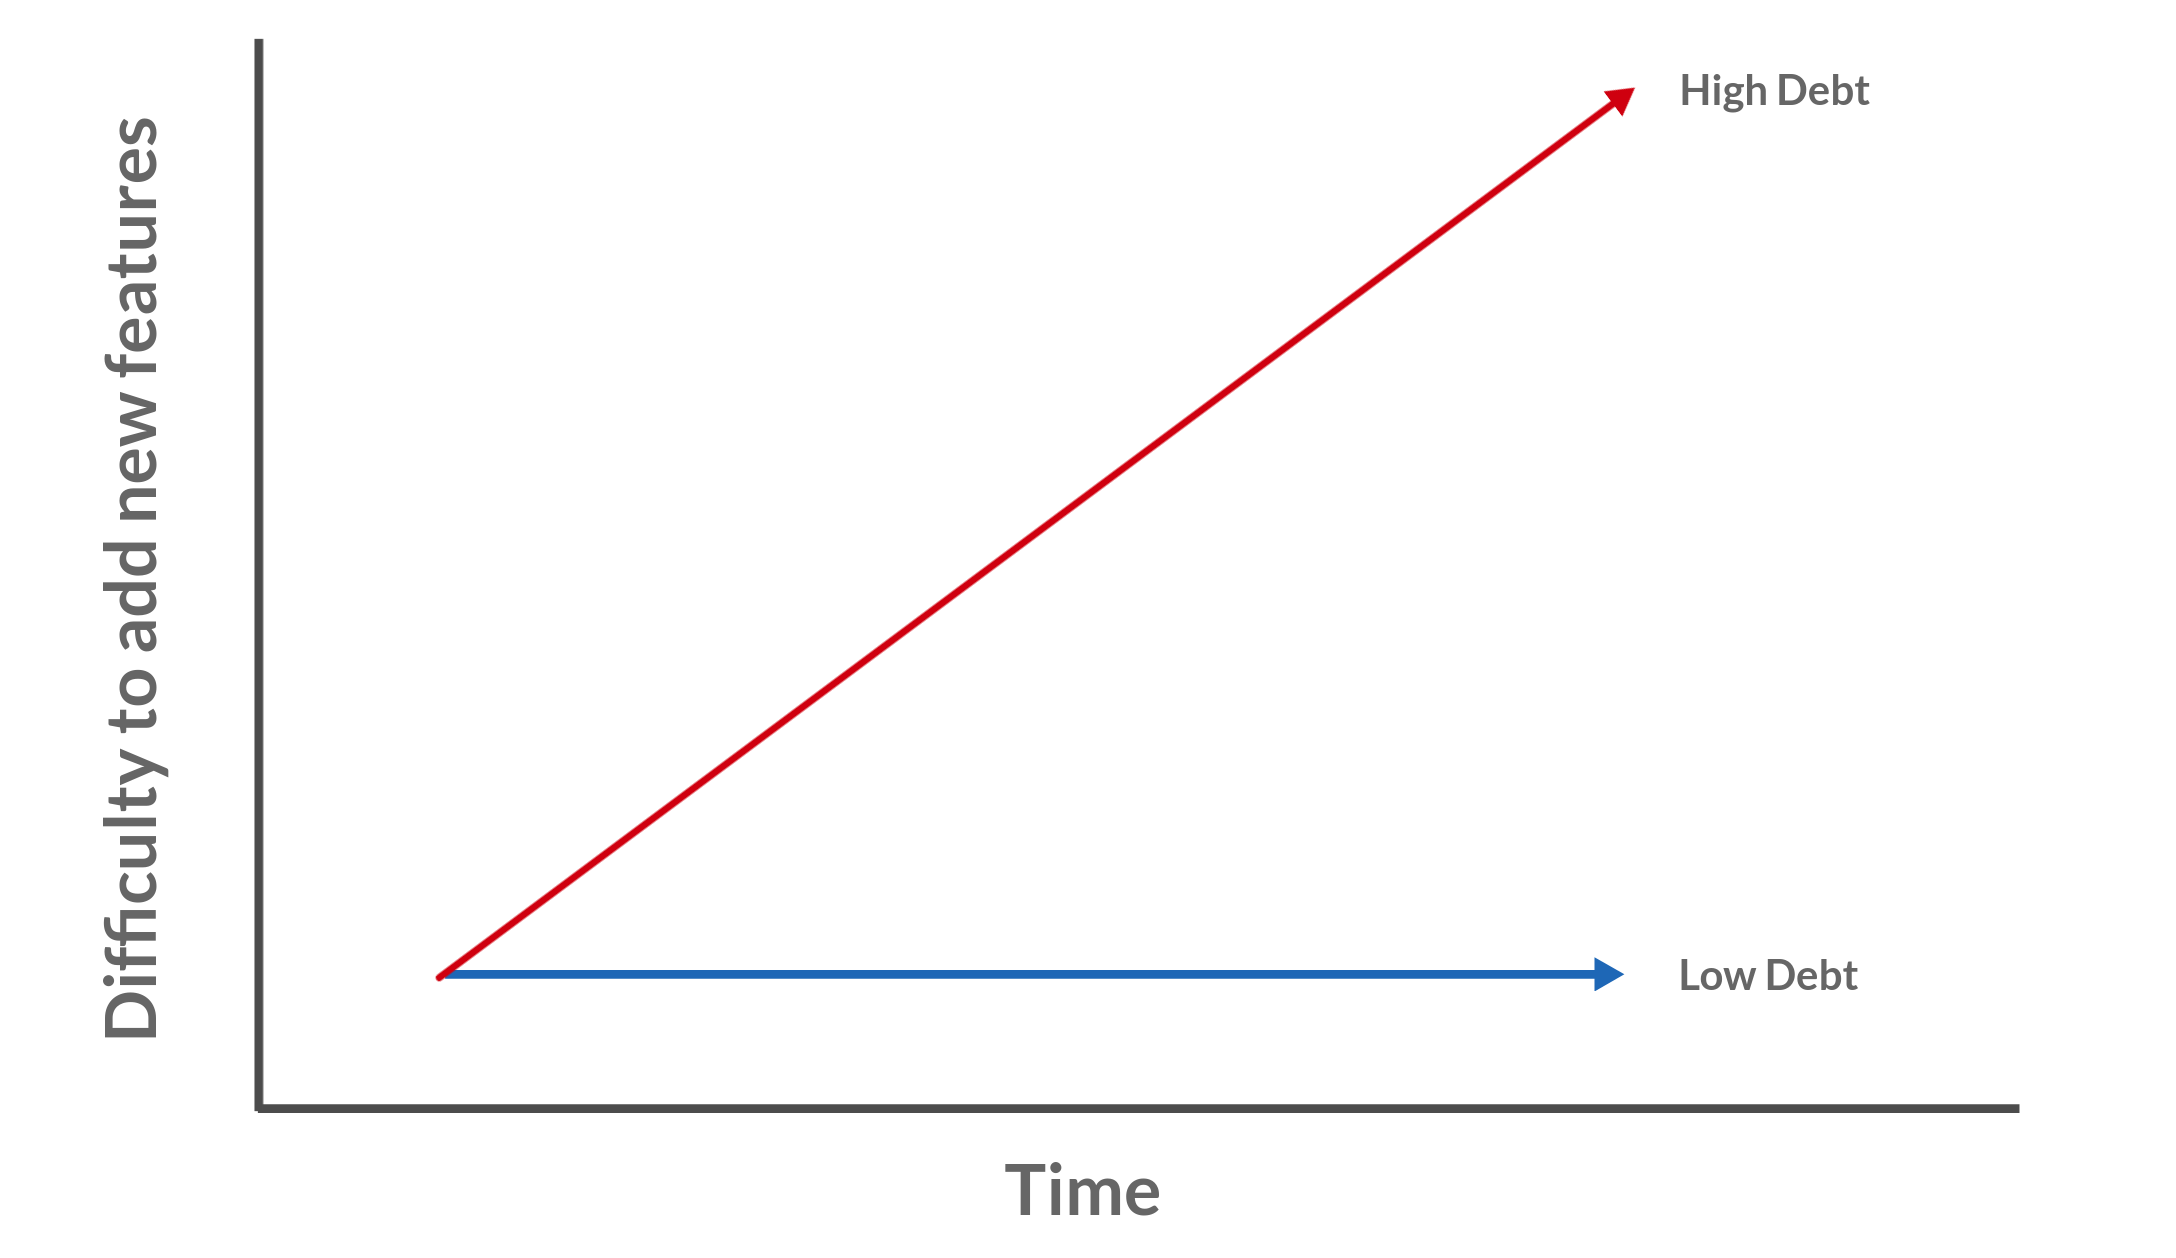
\includegraphics[width=\textwidth]{./assets/technical_debt}
    \caption{Simple depiction of Technical Debt}
\end{figure}

% Technical Debt: Explanation
Technical debt is a helpful metaphor 
	that provides a framework that allows thinking about code smells 
	in terms of financial debt {fowlerdebt}.
In concrete terms, the term Technical debt, coined by Ward Cunningham, describes the extra effort it takes to add new features (\cite{kruchten2012}). 
In financial terms, the additional effort is the interest that has to be paid on the debt (\cite{fowlerdebt}). 
Fowler {fowlerdebt} presents the example 
	of a confusing module structure in a code base.
He illustrates that 
	a programmer could need four days to add new features 
	with a clear structure and six days with code smells. 
Then, the two additional days is the interest a company has paid on the debt.
We see that a company can either decide to pay the interest on technical debt, 
	or reduce it by means of refactoring. 
Within the context of our thesis,
	when referring to technical debt, it is implied code smells are the subject of discussion.
In practice, however, Technical debt must not be limited to code smells. The overarching metaphor of Technical debt encompasses anything 
	that adds friction from software development endeavors (\cite{kruchten2012}). 

% Technical Debt: Unavoidable
One approach to think about solutions is to argue for investing in experienced programmers to avoid debt entirely. 
A company could then do such an undertaking, if the additional money spent on the salaries is offset by the cost endured from debt.
In practice, it is not that simple, as technical debt will always accrue, even with experienced programmers. For instance, sometimes debt accumulates because one quality attribute gained in importance, but the code did not change. Other times it could just be due to the fact that code base exists for a very long time. In both cases, refactoring can be a crucial mechanism in order to get rid of acquired technical debt. 

% Paradox
There can be instances where technical debt is substantial enough, 
	where associated interest payments can not be handled. 
In some cases, it might be more cost-effective to 
	rewrite an entire code bases instead of refactoring it.  
As a consequence, it becomes apparent, that businesses have financial incentives to make the right decisions in order to efficiently allocate their resources.
Such difficult decisions require 
	competent employees that on the one hand know in what ways to deal with the debt, but more importantly to prevent such cases from happening completely.
These employees are not confined to one type of job
As a consequence, lacking the relevant expertise in either management or software engineering departments can lead to undesirable financial ramifications. 
Such conclusions encourage us to look at refactoring from a business standpoint. As a consequence, the section below will explore this topic even further.

\section{Communication Device}
% Economic Context
Being aware of the financial relationship, 
	we see that refactoring must not be restricted to programmers and can be much more relevant to upper team leaders, or product managers.
Having knowledge of abstract concepts, like technical debt,
	allows employees from other domains
	to make decisions and communicate them, without any programming experience.
It can be extremely freeing not to rely on moral principles, 
	but instead provide an evaluation that an also be defended from a business standpoint.
Moreover, some might even argue that decisions regarding refactoring should be purely economic.
Fowler [p.~57]{fowler2018} claims 
	that it is beneficial to have this attitude and argues that economic benefits
	should always be the driving factor of refactoring.

% Communication Device
As alluded to above, Technical debt can also be used as a communication device. 
It is a simple model to form economic decisions, 
	that are potentially very complex.
This device can be used in two directions, top-down or bottom-up.
Top-down communication by experienced team leaders 
	using the term technical debt provides directions to their team members.
As an example, management has decided to migrate their systems to the cloud, 
	but it is realized that the code contains a lot of code smells, 
	which makes it hard to undergo such a change. 
Consequently, by communicating this issue in regard to having too much technical debt in that specific domain.
This aids employees in knowing the particular area 
	to focus on, and prevents them to refactor at places 
	that do not directly contribute to the migration.

% Bottom-up
Additionally, technical debt as a metaphor 
	can also support bottom-up communication.
This metaphor can be used to provide sufficient arguments for refactoring, 
	when clients or upper management are in doubt.
For instance, it could serve as a tool to reason about 
	the difficulties of adding new features or 
	the issues of making major changes to the application. 
As a result, barrier are reduced between 
	software engineers, other departments, and clients, when discussing the 
	underlying problem of code smells. 
Furthermore, with proper communication, 
	clients, for instance, might even be encouraged to further reduce 
	technical debt in order for the software to be adaptive to 
	upcoming trends or customer requests. 
Moreover, keeping technical debt low prevents clients from destroying current value 
	and keep their product to stay successful over the long term.
